\documentclass[tikz,border=8pt]{standalone}
% Shared look for every TikZ diagram. Load with \input{../../tools/tikz-style.tex}
\usepackage[T1]{fontenc}
\usepackage{lmodern}
\renewcommand{\sfdefault}{lmr}  % diagrams use the same serif as the text
\usetikzlibrary{arrows.meta, positioning, shapes.geometric, calc, fit, backgrounds}
\definecolor{cblue}{HTML}{4C78A8}
\definecolor{corange}{HTML}{F58518}
\definecolor{cgreen}{HTML}{54A24B}
\definecolor{cred}{HTML}{E45756}
\definecolor{cpurple}{HTML}{B279A2}
\definecolor{cgrey}{HTML}{6B6B6B}
\tikzset{
  every picture/.style={font=\sffamily, line width=1.2pt},
  box/.style={draw=#1, fill=#1!12, rounded corners=4pt, align=center, inner sep=7pt, minimum height=1.1cm},
  box/.default=cgrey,
  arrow/.style={-{Stealth[length=3mm]}, draw=cgrey, line width=1.4pt},
  title/.style={font=\sffamily\bfseries\Large},
  note/.style={font=\sffamily\small, text=cgrey, align=center},
}
\AtBeginDocument{\hyphenpenalty=10000 \exhyphenpenalty=10000}

\begin{document}
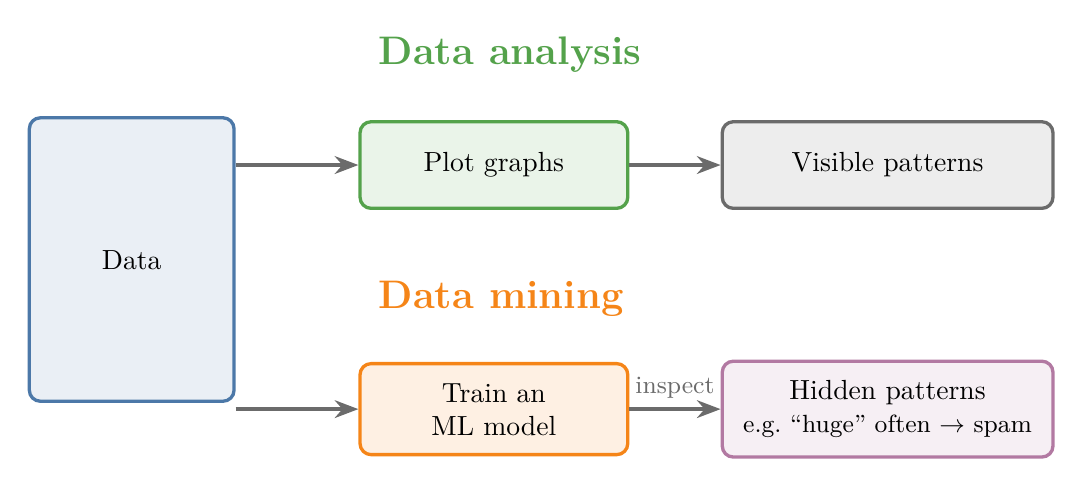
\begin{tikzpicture}
  \node[box=cblue, minimum width=2.6cm, minimum height=3.6cm] (d) at (0,0) {Data};
  % data analysis
  \node[title, cgreen, anchor=west] at (3.0,2.6) {Data analysis};
  \node[box=cgreen, minimum width=3.4cm] (g) at (4.6,1.2) {Plot graphs};
  \node[box=cgrey, minimum width=4.2cm] (v) at (9.6,1.2) {Visible patterns};
  \draw[arrow] (d.east |- g) -- (g); \draw[arrow] (g) -- (v);
  % data mining
  \node[title, corange, anchor=west] at (3.0,-0.5) {Data mining};
  \node[box=corange, minimum width=3.4cm] (m) at (4.6,-1.9) {Train an\\ML model};
  \node[box=cpurple, minimum width=4.2cm] (h) at (9.6,-1.9) {Hidden patterns\\{\small e.g.\ ``huge'' often $\rightarrow$ spam}};
  \draw[arrow] (d.east |- m) -- (m); \draw[arrow] (m) -- node[note, above]{inspect} (h);
\end{tikzpicture}
\end{document}
